\documentclass[10pt, hyperref={pdfpagelabels=false}]{beamer}

\usepackage{tikz, verbatim, enumitem}

\usetikzlibrary{decorations}
\usetikzlibrary{backgrounds}
\usetikzlibrary{patterns}
\usetikzlibrary{snakes}
\usetikzlibrary{shapes}
\usetikzlibrary{positioning, shapes.geometric, arrows.meta}
\usetikzlibrary{arrows,automata}

\setlength{\parindent}{0pt}
\setlength{\parskip}{1.3ex}

\title{State Machines}
\author{Michael Brockway}
\date{\today}

\setlist[enumerate]{itemsep=0mm}
\setitemize{label=\usebeamerfont*{itemize item}
  \usebeamercolor[fg]{itemize item}
  \usebeamertemplate{itemize item}}

\begin{document}

\begin{frame}
\titlepage
\end{frame}

\begin{frame}
\frametitle{A control system example}
Suppose you have to write software for an industrial system. A simple example is one comprising a conveyor belt, a robot arm that picks items up from an input area and puts then on the the belt, and another robot arm that removes them from the far end of the belt.

The three components have their own control software but a emph{supervisory unit} needs to coordinate their actions. In particular,
\begin{itemize}
\item When starting the system up, it needs to know when each of the other components is ready to act;
\item When shutting the system down it needs to know there are no items part-way through the system;
\item It needs to be able to tell the input robot there is an item to pick up;
\item It needs to know when the output robot has removed an item from the belt;
\item It needs to be able to pause the system and resume operation;
\item It needs to halt the system in case of emergency.
\end{itemize}
\end{frame}

\begin{frame}
\frametitle{A control system example}
To design software for this, think of the system being in one of a set of \emph{states}:
\begin{center}
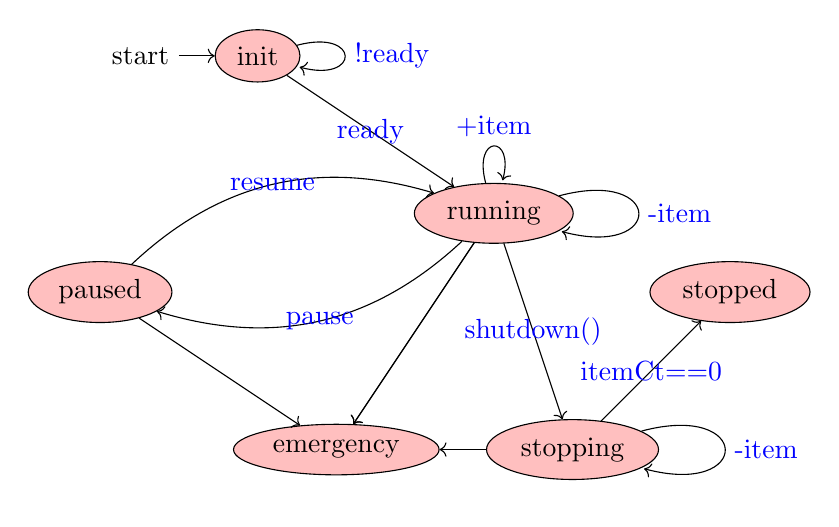
\begin{tikzpicture} [ball/.style={ellipse, minimum width=2, minimum height=1, draw, >=stealth}]
  \draw (0,2)   node[initial, ball, fill=pink](ini)  {init}; 
  \draw (3,0)   node[ball, fill=pink](rng) {running};
  \draw (-2,-1)  node[ball, fill=pink](psd) {paused};
  \draw (4,-3)   node[ball, fill=pink](stpg) {stopping};
  \draw (6,-1)   node[ball, fill=pink](stpd) {stopped};
  \draw (1,-3) node[ball, fill=pink](em) {emergency};

\path (ini) edge[loop right] node {\color{blue}!ready} (ini)
            edge[->] node {\color{blue}ready} (rng)
      (rng) edge[->] (em)
            edge[->] node {\color{blue}shutdown()} (stpg)
            edge[->, bend left] node {\color{blue}pause} (psd) 
            edge[loop above] node{\color{blue}+item} (rng)
            edge[loop right] node{\color{blue}-item} (rng)
            edge[->] (em)
     (stpg) edge[loop right] node{\color{blue}-item} (stpg)
            edge[->] node{\color{blue}itemCt==0} (stpd)
            edge[->] (em)
      (psd) edge[->, bend left] node {\color{blue}resume} (rng)
            edge[->] (em);
\end{tikzpicture}
\end{center}
\end{frame}

\begin{frame}
\frametitle{A control system example}
The states are
\begin{itemize}
\item {\color{brown} \large init running paused stopping stopped emergency}
\item {\color{brown} init} is the \emph{initial} state.
\end{itemize}

\emph{Transitions} between states are denoted by labelled arrows
\begin{itemize}
\item The labels may denote \emph{events} or \emph{actions} or \emph{conditions}
\item {\color{blue}!ready} means the components have not all notified that they are ready; once they have ({\color{blue}ready} event) the system goes to {\color{brown}running} state.
\item {\color{blue}+item} means an item has entered the system; {\color{blue}-item} means an item has been delivered by the system;
\item {\color{blue}itemCt==0} means all items have been delivered; there are none left in the system, so the system tranfers to the  {\color{brown}stopped} state. Counter \texttt{itemCt} is  programmed to keep track of this.
\end{itemize}
\end{frame}

\begin{frame} [fragile]
\frametitle{A control system example}
In general, the behaviour you have to program is dependent on the state of the system. There you tend to write such constructs as
{\color{blue}
\begin{verbatim}
if (state == init} {
  if (allComponentsReady())   { state = idle; }
}
else if (state == running)  {
  if (pause())                { state = paused; }
  else if (itemArrived())     { itemCt++; }
  else if (itemDelivered())   { itemCt--; }
  else if (shutdown())        { state = stopping; }
}
else if (state == stopping) {
    if (itemCt==0)            { state = stopped; }
    else if (itemDelivered()) { itemCt--;  }
}
else  ...
\end{verbatim}
}
\end{frame}

\begin{frame} [fragile]
\frametitle{A control system example}
Another coding style is to use the \texttt{switch} construct ...
{\color{blue}
\begin{verbatim}
switch (state) {
  case init:
    if (allComponentsReady())   { state = idle; }
    break;
  case running:
    if (pause())                { state = paused; }
    else if (itemArrived())     { itemCt++; }
    else if (itemDelivered())   { itemCt--; }
    else if (shutdown())        { state = stopping; }
    break;
  case stopping:
    if (itemCt==0)            { state = stopped; }
    else if (itemDelivered()) { itemCt--;  }
    break;
  .... (more cases)
} 
\end{verbatim}
}
\end{frame}

\begin{frame}
Note that labels on transitions to state {\color{brown}emergency} have been omitted from the diagram to save clutter. There would be cases correpsonding to these too.

The 'philosophy' of state machines such as this is that
\begin{itemize}
\item the system in some particular state will always try to move via a transition so another state.
\item If it cannot that sytem is \emph{deadlocked}.
\end{itemize}

The transition labels indicate \emph{events} that trigger change of state and/or an update of state variables.
\begin{itemize}
\item This might be an external event:
  \begin{itemize}
  \item an input from a sensor or the network;
  \item an interrupt
  \end{itemize}
\item ... or just some predicate on the state variable (eg \texttt{\color{blue}itemCt == 0}) becomong \texttt{\color{blue}true}.
\end{itemize}
\end{frame}

\begin{frame}
\frametitle{Vending machine example}
Another imformal example is a vending machine which
\begin{itemize}
\item allows the customer to choose quantities of each of a number of wares,
\item will accept payment by cash or card, and
\item dispense the goods at the conclusion of payment.
\end{itemize}

If you were developing the software for this machine you might find a state machine like the following useful.
\end{frame}

\begin{frame}
\frametitle{Vending machine example}
\begin{center}
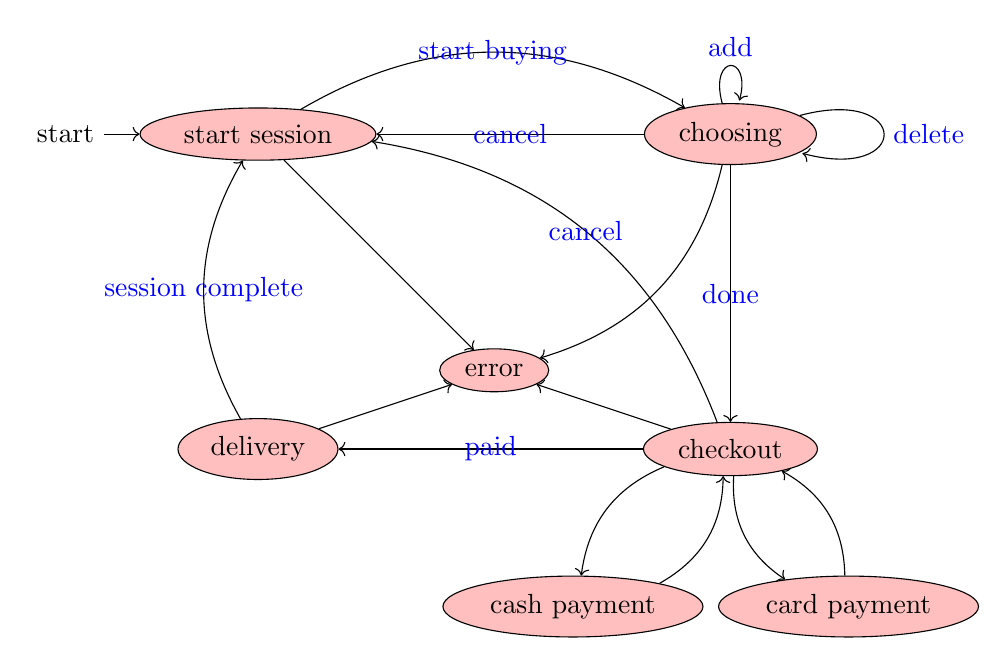
\begin{tikzpicture} [ball/.style={ellipse, minimum width=2, minimum height=1, draw, >=stealth}]
  \draw (-2,3)   node[initial, ball, fill=pink](ini)  {start session}; 
  \draw (4,3)   node[ball, fill=pink](cng) {choosing};
  \draw (4,-1)  node[ball, fill=pink](chk) {checkout};
  \draw (5.5,-3)   node[ball, fill=pink](crd) {card payment};
  \draw (2,-3)   node[ball, fill=pink](csh) {cash payment};
  \draw (-2,-1)   node[ball, fill=pink](dlvy) {delivery};
  \draw (1,0) node[ball, fill=pink](err) {error};

\path (ini) edge[->, bend left] node {\color{blue}start buying} (cng)
            edge[->] (err)
      (cng) edge[->] node {\color{blue}done} (chk)
            edge[loop above] node{\color{blue}add} (cng)
            edge[loop right] node{\color{blue}delete} (cng)
            edge[->, bend left] (err)
            edge[->] node {\color{blue}cancel} (ini)
      (chk) edge[->, bend right] (crd)
            edge[->, bend right] (csh)
            edge[->] node {\color{blue}paid}(dlvy)
            edge[->] (err)
            edge[->, bend right] node {\color{blue}cancel} (ini)
     (dlvy) edge[->, bend left] node {\color{blue}session complete} (ini)
            edge[->] (err)
      (csh) edge[->, bend right] (chk)
      (crd) edge[->, bend right] (chk);
\end{tikzpicture}
\end{center}
\end{frame}

\begin{frame}
\frametitle{Vending machine example}
Exercises for you -
\begin{itemize}
\item Describe the significance of each of the states.
\item Describe the significance of each of the transition labels.
\item Suggest labels for the transitions between `checkout' and `cash payment', `card payment' and describe their significance.
\item Write pseudocode for (some of) the diagram.
\item Can you extend the state machine to include accepting coins/notes? giving change?
\end{itemize}
\end{frame}

\begin{frame}
\frametitle{More formal state machines}
This way of depicting 'computational logic' has been around for a while. 

A related idea, \emph{flow charts} \href{https://en.wikipedia.org/wiki/Flowchart}{\textcolor{blue}{[wiki]}} have been around since the 1950s or longer.
\begin{itemize}
\item The basic flow-chart is very simple: a start-point, end- or exit-points, rectangles denoting activities and diamond-shaped boxes denoting decisions.
\item Program logic was depicted on flow charts in the early years but this became unwieldy very quickly.
\end{itemize}

A more sophisticated formal construct, the \emph{finite state automaton} (or \emph{finite state machine}, FSA or FSM if you like TLAs\footnote{three-letter acronyms}) has been very useful in theoretical computing science, and continues to be.
\end{frame}

\begin{frame}
\frametitle{Finite-state automata}
A finite-state automaton is based on a finite set $A$ of symbols or \emph{letters}, called its \emph{alphabet}. It is a construct $(Q, R, q_0, F)$ where
\begin{itemize}
\item $Q$ is a (finite, non-empty) set of \emph{locations} or \emph{states};
\item $q_0$ is a particular ($q_0 \in Q$) \emph{initial state};
\item $R$ is a set of \emph{edges} between pairs of states, labelled with letters from $A$. A typical edge is something like $q_1 \stackrel{a}{\longrightarrow} q_2$ where $a \in A$ and $q_1, q_2 \in Q$.
\item $F \subseteq Q$. $F$ is a particular subset of states, \emph{final} states.
\end{itemize} 

We have seen two (almost) examples already: the control system model and the vending machine model. Here, $Q$ is the set of states, $q_0$ the intial state, $A$ the set of events or actions that label the arrows, and $R$ the labelled arrows themselves. 

For more (similar) examples see the \href{https://en.wikipedia.org/wiki/Finite-state_machine}{\textcolor{blue}{[wiki]}}
\end{frame}

\begin{frame}
\frametitle{Finite-state automata}
A \emph{run} of an automaton is a sequence of locations/states starting with the initial state $q_0$ and with each state in the sequence connected to the previous state by an edge labelled by an element of $A$. Thus A, for 'alphabet' could also stand for 'actions'. An automaton is
\begin{itemize}
\item \emph{deterministic} if from any state, there is at most one transition available to a 'next state, and
\item \emph{non-deterministic} otherise: from some states there is a choicde of 'next' actions.
\end{itemize}

A early use of finite-state automata in theoretical computing science was to define a \emph{language} over an alphabet, $A$. 
\begin{itemize}
\item Take a string of symbols from $A$, $a_1a_2a_3...a_n$ and present this as 'input' to an automaton $(Q, R, q_0, F)$. 
\item Let the automaton run, 'consuming' a letter each time it takes a transition: 
\item ... so the run will look something like $q_0 \stackrel{a_1}{\longrightarrow} q_1\stackrel{a_2}{\longrightarrow} q_2\stackrel{a_3}{\longrightarrow}q_3\stackrel{a_4}{\longrightarrow} ... \stackrel{a_n}{\longrightarrow} q_2$. 
\end{itemize}
\end{frame}

\begin{frame}
\frametitle{Finite-state automata}
If a run is possible in which $q_n \in F$, that is, it ends up in a state in the special subset $F$, we say the automaton \emph{accepts} the string.

An early theoretical result was if $A$ is the 'ordinary' alphabet, then the strings of letters from $A$ accepted by FSMs are exactly the \emph{regular expressions}.

Interestingly, this is the same whether we restrict to deterministic automata, or allow non-deterministic ones too. We can also allow runs to include transitions with an 'empty' label, but we still get just the reqular expressions.
\end{frame}

\begin{frame}
\frametitle{Timed automata}
In one of our final-year modules, embedded system specification and design, we employ this further development of the finitate-state automaton, in which
\begin{itemize}
\item the automaton has a set of 'stop-clocks' which 'tick' at a regular rate during a run. 
\item A state/location can be specified to accessible only if the time on a clock is $\le$ some value, and 
\item the transitions/edges are decorated with 
  \begin{itemize}
  \item \emph{guards} which allow the transition only if some test on the clocks is satisfied, and also with
  \item  \emph{actions} with reset clocks and perform other updates to system variables when the transtion is taken during a run.
  \end{itemize}
\end{itemize}

This turns out to be a powerful technique for modelling and testing the behaviour of real-time 
\end{frame}

\begin{frame}
\frametitle{Probabilistic automata}
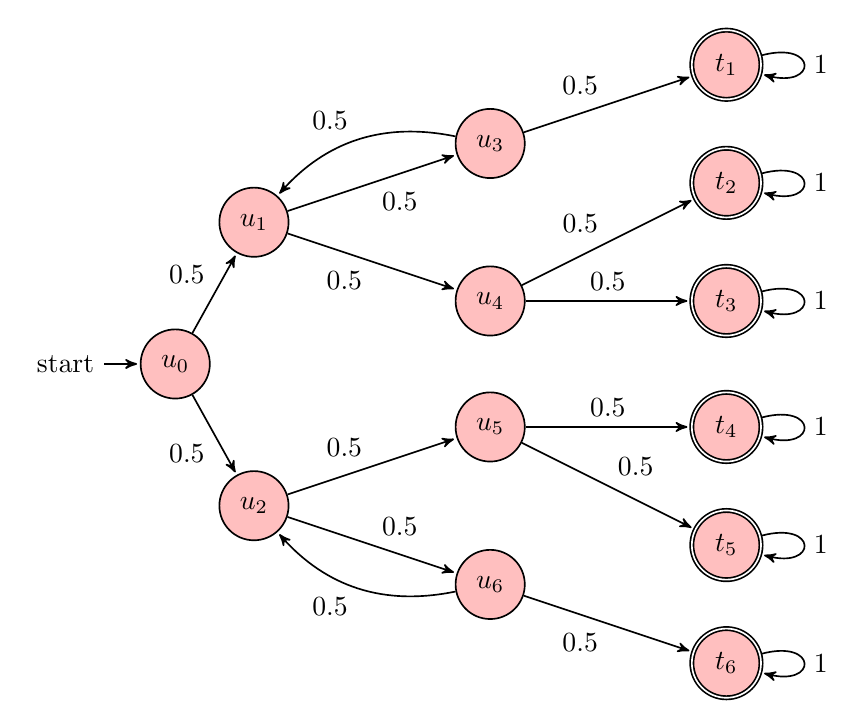
\begin{tikzpicture}[->,>=stealth',shorten >=1pt,auto,semithick]
  \tikzstyle{every state}=[fill=pink,text=black]

  \node[initial,state] (U0) at (0,0)    {$u_0$};
  \node[state]         (U1) at (1,1.8)  {$u_1$};
  \node[state]         (U2) at (1,-1.8) {$u_2$};
  \node[state]         (U3) at (4,2.8)  {$u_3$};
  \node[state]         (U4) at (4,0.8)  {$u_4$};
  \node[state]         (U5) at (4,-0.8) {$u_5$};
  \node[state]         (U6) at (4,-2.8) {$u_6$};
  \node[state, accepting] (T1) at (7,3.8)  {$t_1$};
  \node[state, accepting] (T2) at (7,2.3)  {$t_2$};
  \node[state, accepting] (T3) at (7,0.8)  {$t_3$};
  \node[state, accepting] (T4) at (7,-0.8) {$t_4$};
  \node[state, accepting] (T5) at (7,-2.3) {$t_5$};
  \node[state, accepting] (T6) at (7,-3.8) {$t_6$};

  \path (U0) edge node {0.5} (U1)
             edge [swap] node {0.5} (U2)
        (U1) edge [swap] node {0.5} (U3)
             edge [swap] node {0.5} (U4)
        (U2) edge node {0.5} (U5)
             edge node {0.5} (U6)
        (U3) edge node {0.5} (T1)
             edge [swap, bend right] node {0.5} (U1)
        (U4) edge node {0.5} (T2)
             edge node {0.5} (T3)
        (U5) edge node {0.5} (T4)
             edge node {0.5} (T5)
        (U6) edge [swap] node {0.5} (T6)
             edge [bend left] node {0.5} (U2)
        (T1) edge [loop right] node{1}(T1)
        (T2) edge [loop right] node{1}(T2)
        (T3) edge [loop right] node{1}(T3)
        (T4) edge [loop right] node{1}(T4)
        (T5) edge [loop right] node{1}(T5)
        (T6) edge [loop right] node{1}(T6);
\end{tikzpicture}
\end{frame}

\begin{frame}
\frametitle{Probabilistic automata}
Another interesting devlopement of the basic finite automaton is a state machine in which the transitions between states/locations are decorated with \emph{probabilities}.
\begin{itemize}
\item Each state has a set of forward transitions with probablities adding up to 1. 
\item In a run, the transition with probability $p$ is selected, with probability $p$.
\end{itemize}

In the example above (due to Knuth and Yao), each state has two transitions outward and a run takes one transition or the other with a 50-50 chance - a toss of a coin.
\begin{itemize}
\item The probability of reaching state $t_2$ is $(\frac{1}{2})^3 + (\frac{1}{2})^5 + (\frac{1}{2})^7 + (\frac{1}{2})^9 + ... = (\frac{1}{2})^3 (1 + \frac{1}{4} + \frac{1}{16} + \frac{1}{64} + ...) = \frac{1}{8} \times \frac{4}{3} = \frac{1}{6}$
\item In fact the same calculation applies to all the $t_n$ states.
\end{itemize}
A roll of a 6-sided die is simulated with coin tosses!
\end{frame}

\begin{frame}
\frametitle{State diagrams and the state design pattern}
Not surprisingly, UML has a version of state machines: see, for instance, \href{http://www.agilemodeling.com/artifacts/stateMachineDiagram.htm}{\textcolor{blue}{agilemodeling.com}}
\begin{itemize}
\item These \emph{state charts} can be hierarchical, as in figure two on the Agile Modelling page: a state can be made up of a 'miniature' state machine.
\end{itemize}

Lastly, again another object-oriented view of state machines is given by the \emph{state design pattern}: see, for example the \href{https://en.wikipedia.org/wiki/State_pattern}{\textcolor{blue}{State pattern wiki}}
\begin{itemize}
\item This design pattern really formalises the system for coding a state-driven system like the examples we began with.
\item Formally, there is a choice of functionalities dependent on state. In C this used be done with an array of pointers to functions indexed by the state. In a modern OO language like java, the different (polymorphic) functionalities would be in classes implementing a common interface and the state would determine a particular implementation.
\end{itemize}
\end{frame}

\end{document}

